\documentclass{article}
\usepackage{tikz,geometry}
\usetikzlibrary{arrows,positioning,calc}
\usepackage[T1]{fontenc}
\usepackage[utf8]{inputenc}
\pagestyle{empty}
\geometry{
paperwidth=14cm,
paperheight = 8cm,
left=0pt,
right=0pt,
top=2pt,
bottom=0pt
}
\begin{document}
\centering
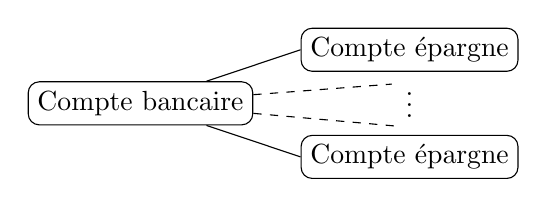
\begin{tikzpicture}[every node/.append style={align=left,draw,rounded corners}]
\node (bank) at (0,0) {Compte bancaire};
\node[above right=4mm and 6mm] (epa1)  at (bank.east) {Compte épargne};
\node[below right=4mm and 6mm] (epa2)  at (bank.east) {Compte épargne};
\node[draw=none] at ( $(epa1.south)!0.4!(epa2.north)$ ) {$\vdots$};
\foreach \i in {10,-10}
  \draw[dashed] (bank) -- ( $(bank)!0.9!\i:(epa1.south)!0.5!(epa2.north)$);
\foreach \i in {1,2}
  \draw (bank) -- (epa\i.west);
\end{tikzpicture}
\end{document}
